% $Header: /Users/joseph/Documents/LaTeX/beamer/solutions/conference-talks/conference-ornate-20min.en.tex,v 90e850259b8b 2007/01/28 20:48:30 tantau $

\documentclass[xcolor={usenames,dvipsnames}]{beamer}

% This file is a solution template for:

% - Talk at a conference/colloquium.
% - Talk length is about 20min.
% - Style is ornate.



% Copyright 2004 by Till Tantau <tantau@users.sourceforge.net>.
%
% In principle, this file can be redistributed and/or modified under
% the terms of the GNU Public License, version 2.
%
% However, this file is supposed to be a template to be modified
% for your own needs. For this reason, if you use this file as a
% template and not specifically distribute it as part of a another
% package/program, I grant the extra permission to freely copy and
% modify this file as you see fit and even to delete this copyright
% notice. 


\mode<presentation>
{
  \usetheme{Copenhagen}
  \usecolortheme{dolphin}
}
  % or ...

  \setbeamercovered{transparent}
  % or whatever (possibly just delete it)


\usepackage[percent]{overpic}
\usepackage[english]{babel}
\usepackage{setspace}
\usepackage{comment}
\usepackage[makeroom]{cancel}
\usepackage[absolute,overlay]{textpos}
% or whatever

\usepackage[latin1]{inputenc}
% or whatever

\usepackage[at]{easylist}
\usepackage{times}
\usepackage[T1]{fontenc}
\usepackage{xcolor}
% Or whatever. Note that the encoding and the font should match. If T1
% does not look nice, try deleting the line with the fontenc.

\definecolor{darkestblue}{RGB}{1,8,100}
\definecolor{darkerblue}{RGB}{3,17,150}
\definecolor{darkblue}{RGB}{7,26,200}
\definecolor{lightred}{RGB}{202,103,104}
\definecolor{lightgreen}{RGB}{106,202,107}

%particles
\newcommand{\jpsi}{\rm J/$\psi$}
\newcommand{\psip}{$\psi^\prime$}
\newcommand{\jpsiDY}{\rm J/$\psi$\,/\,DY}
\newcommand{\chic}{$\chi_{\rm c}$}
\newcommand{\pip}{$\pi^{+}$}
\newcommand{\pim}{$\pi^{-}$}
\newcommand{\pizero}{$\pi^{0}$}
\newcommand{\kap}{K$^{+}$}
\newcommand{\kam}{K$^{-}$}
\newcommand{\pbar}{$\rm\overline{p}$}
\newcommand{\ccbar}{\ensuremath{\mathrm{c\overline{c}}}}
\newcommand{\bbbar}{\ensuremath{\mathrm{b\overline{b}}}}
\newcommand{\Dzero}{\ensuremath{\mathrm{D^{0}}}}
\newcommand{\Dzerobar}{\ensuremath{\mathrm{\overline{D}^{0}}}}
\newcommand{\Dpm}{\ensuremath{\mathrm{D^{\pm}}}}
\newcommand{\Ds}{\ensuremath{\mathrm{D_{s}^{\pm}}}}
\newcommand{\Dstar}{\ensuremath{\mathrm{D^{*\pm}}}}

%collision systems
\newcommand{\pp}{pp}
\newcommand{\pPb}{p--Pb}
\newcommand{\PbPb}{Pb--Pb}

%detectors
\newcommand{\ezdc}{$E_{\rm ZDC}$}

%units
\newcommand{\GeVc}{GeV/$c$}
\newcommand{\GeVcsq}{GeV/$c^2$}

%others
\newcommand{\degree}{$^{\rm o}$}
\newcommand{\s}{\ensuremath{\sqrt{s}}}
\newcommand{\snn}{\ensuremath{\sqrt{s_{\rm NN}}}}
\newcommand{\y}{\ensuremath{y}}
\newcommand{\pt}{\ensuremath{p_{\rm T}}}
\newcommand{\dedx}{d$E$/d$x$}
\newcommand{\dndy}{d$N$/d$y$}
\newcommand{\dndydpt}{${\rm d}^2N/({\rm d}y {\rm d}p_{\rm t})$}
\newcommand{\zpar}{\ensuremath{z_{||}}}
\newcommand{\zpargen}{\ensuremath{z_{||}^{\mathrm{part}}}}
\newcommand{\zpardet}{\ensuremath{z_{||}^{\mathrm{det}}}}
\newcommand{\ptchjet}{\ensuremath{p_{\mathrm{T,ch\, jet}}}}
\newcommand{\ptjet}{\ensuremath{p_{\mathrm{T,jet}}}}
\newcommand{\ptchjetgen}{\ensuremath{p_{\mathrm{T,ch\,jet}}^{\mathrm{part}}}}
\newcommand{\ptchjetdet}{\ensuremath{p_{\mathrm{T,ch\,jet}}^{\mathrm{det}}}}
\newcommand{\ptd}{\ensuremath{p_{\mathrm{T,D}}}}
\newcommand{\ptdgen}{\ensuremath{p_{\mathrm{T,D}}^{\mathrm{part}}}}
\newcommand{\ptddet}{\ensuremath{p_{\mathrm{T,D}}^{\mathrm{det}}}}
\newcommand{\antikt}{anti-\ensuremath{k_{\mathrm{T}}}}
\newcommand{\Antikt}{Anti-\ensuremath{k_{\mathrm{T}}}}
\newcommand{\kt}{\ensuremath{k_{\mathrm{T}}}}
\newcommand{\pthard}{\ensuremath{p_{\mathrm{T,hard}}}}

\begin{comment}
\AtBeginSection[]{
  \begin{frame}
  \vfill
  \centering
  \begin{beamercolorbox}[sep=8pt,center,shadow=true,rounded=true]{title}
    \usebeamerfont{title}\insertsectionhead\par%
  \end{beamercolorbox}
  \vfill
  \end{frame}
}
\end{comment}

\setbeamersize{text margin left=15pt,text margin right=15pt} 

\title[Jets and heavy flavor in heavy-ion collisions with ALICE] % (optional, use only with long paper titles)
{New results on jets and heavy flavor in heavy-ion collisions with ALICE}

\author[Salvatore Aiola (Yale University)]% (optional, use only with lots of authors)
{Salvatore Aiola, \\
on behalf of the ALICE Collaboration}
% - Give the names in the same order as the appear in the paper.
% - Use the \inst{?} command only if the authors have different
%   affiliation.

\institute[Yale University] % (optional, but mostly needed)
{  
\includegraphics[height=0.9cm]{img/yale}\quad
    
\includegraphics[height=0.8cm]{img/yale_text}}

\date[May 18th, 2017] % (optional, should be abbreviation of conference name)
{LHCP Conference \\
Shanghai Jiao Tong University, China\\
May 18th, 2017}
% - Either use conference name or its abbreviation.
% - Not really informative to the audience, more for people (including
%   yourself) who are reading the slides online

\newcommand*\oldmacro{}%
\let\oldmacro\insertshorttitle%
\renewcommand*\insertshorttitle{%
   \oldmacro\hfill%
   \insertframenumber\,/\,\inserttotalframenumber}
   
   \addtobeamertemplate{frametitle}{}{%
  \begin{textblock*}{2cm}(11.6cm,0.1cm) % {block width} (coords)
  
\includegraphics[height=1.1cm]{img/alice}
  \end{textblock*}}
  
  \newcommand{\backupbegin}{
   \newcounter{finalframe}
   \setcounter{finalframe}{\value{framenumber}}
}
\newcommand{\backupend}{
   \setcounter{framenumber}{\value{finalframe}}
}


\subject{High-Energy Physics}
% This is only inserted into the PDF information catalog. Can be left
% out. 



% If you have a file called "university-logo-filename.xxx", where xxx
% is a graphic format that can be processed by latex or pdflatex,
% resp., then you can add a logo as follows:

% \pgfdeclareimage[height=0.5cm]{university-logo}{university-logo-filename}
% \logo{\pgfuseimage{university-logo}}


% If you wish to uncover everything in a step-wise fashion, uncomment
% the following command: 

%\beamerdefaultoverlayspecification{<+->}


\begin{document}

\begin{frame}
  \titlepage
  \begin{textblock*}{2cm}(11.6cm,0.1cm) % {block width} (coords)
  
\includegraphics[height=1.1cm]{img/alice}
  \end{textblock*}
  
    \begin{textblock*}{2.2cm}(0.2cm,8.2cm) % {block width} (coords)
  
\includegraphics[height=1.1cm]{img/doe}
  \end{textblock*}
\end{frame}

%\begin{frame}{Outline}
  % \tableofcontents
%\end{frame}


% Structuring a talk is a difficult task and the following structure
% may not be suitable. Here are some rules that apply for this
% solution: 

% - Exactly two or three sections (other than the summary).
% - At *most* three subsections per section.
% - Talk about 30s to 2min per frame. So there should be between about
%   15 and 30 frames, all told.

% - A conference audience is likely to know very little of what you
%   are going to talk about. So *simplify*!
% - In a 20min talk, getting the main ideas across is hard
%   enough. Leave out details, even if it means being less precise than
%   you think necessary.
% - If you omit details that are vital to the proof/implementation,
%   just say so once. Everybody will be happy with that.


%\begin{overpic}[width=\textwidth, trim=0 0 0 0, clip]{img/823_D0_Charged_R040_JetPtBins_DPt_30}
%\end{overpic}

%\begin{columns}
%\column{0.5\textwidth}
%\column{0.5\textwidth}
%\end{columns}

\section{Introduction}

\begin{frame}{ALICE}
\begin{columns}

\column{.58\textwidth}
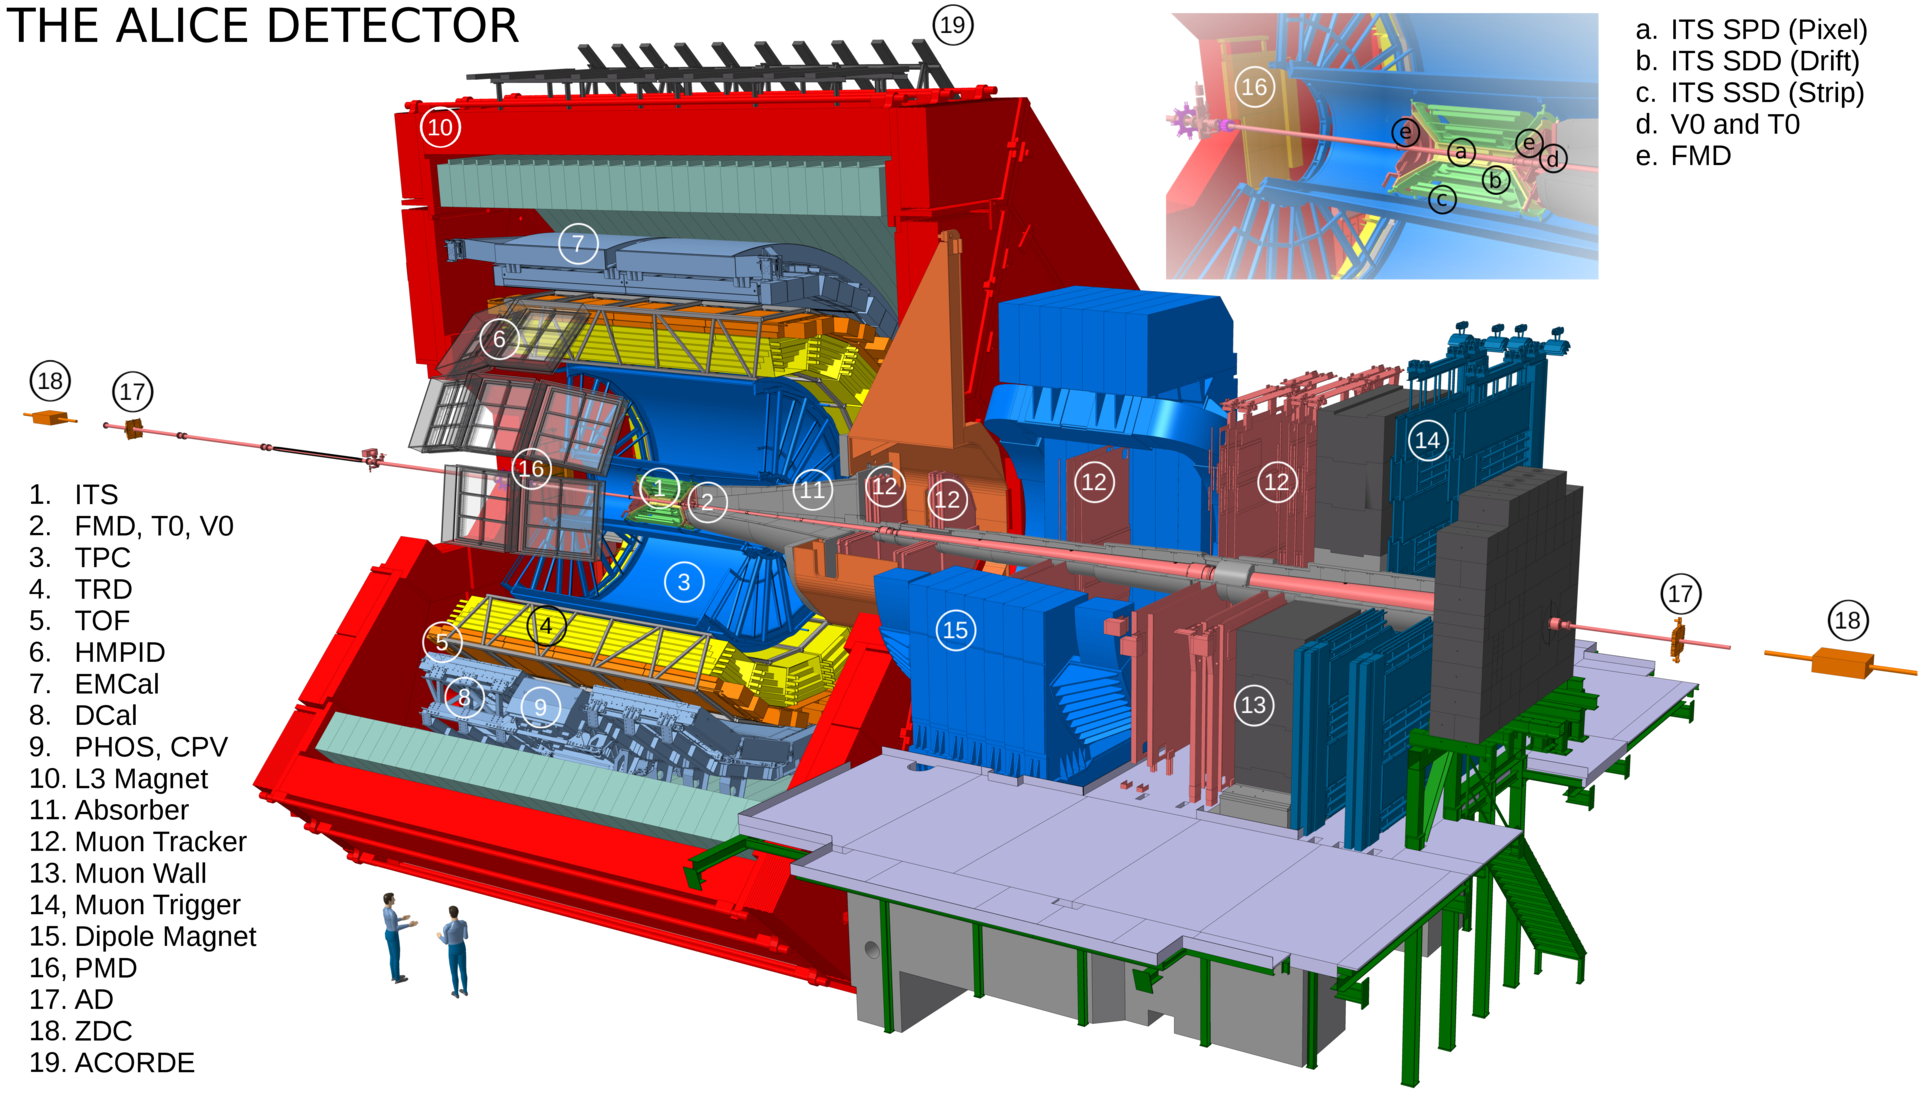
\includegraphics[width=\textwidth]{img/ALICE_Schematics}

\column{.42\textwidth}
\small
\begin{itemize}
\item \alert{D mesons} via hadronic decays (ITS, TPC, TOF)
\begin{itemize}
\item PID, topological cuts
\item invariant mass analysis
\end{itemize}
\item Semileptonic decays of heavy-flavor hadrons
\begin{itemize}
\item \alert{e$^{\pm}$} (TPC, TOF, EMCal)
\item \alert{$\mu^{\pm}$} (muon arm)
\end{itemize}
\end{itemize}
\end{columns}
\begin{itemize}
\item \alert{Jet reconstruction} using \antikt\ algorithm
\begin{itemize}
\item \textcolor{ForestGreen}{charged constituents} (ITS, TPC) $\rightarrow$ \emph{charged jets}
\item add \textcolor{NavyBlue}{neutral constituents} (EMCal, DCal) $\rightarrow$ \emph{full jets} 
\end{itemize}
\end{itemize}
\end{frame}

\begin{frame}{Jets}
\begin{columns}
\column{0.5\textwidth}
\begin{overpic}[width=\textwidth, trim=0 0 0 0, clip]{img/jets/2016-Sep-22-Jet_RAACent}
\end{overpic}
\column{0.5\textwidth}
\small
\begin{itemize}
\item Nuclear modification factor:\\
\vspace{4pt}
$R_{\rm AA} = \frac{\mathrm{d}N_{\rm AA} / \mathrm{d}\pt}{\langle N_{\rm coll} \rangle \mathrm{d}N_{\rm\pp} / \mathrm{d}\pt}$
\item Jets are \alert{strongly suppressed} in \PbPb\ collisions compared to scaled \pp
\item Parton \alert{energy loss} in the QGP
\end{itemize}
\end{columns}
\begin{itemize}
\item Where does the energy go?
\item Is the internal structure of the jet modified?
\item What is the energy loss mechanism?
\end{itemize}
\end{frame}

\begin{frame}[fragile]{Heavy-Flavor}
\begin{columns}
\column{0.4\textwidth}
\begin{overpic}[width=\textwidth, trim=0 0 0 0, clip]{img/hf/2015-Sep-24-AverageDmesonRaavspT_Pions_Nch_010}
\put(30,40){\tiny \href{http://doi.org/10.1007/JHEP03(2016)081}{JHEP 03 (2016) 081}}
\end{overpic}
\column{0.6\textwidth}
\small
\begin{itemize}
\item Charm and beauty produced in \alert{high-$Q^{2}$ processes}
\item Produced early in the collision $\rightarrow$ \alert{experience medium evolution}
\item Negligible thermal production in the QGP ($m_{\rm c,b}\gg T_{\rm QGP}$)
\end{itemize}
\end{columns}
\small
\begin{itemize}
\item Thermalization in the QGP at low \pt
\item Energy loss in the QGP at hight \pt
\begin{itemize}
\item Color charge (Casimir factor): $\Delta E_{\rm q} < \Delta E_{\rm g}$
\item Dead cone effect (radiative energy loss): $\Delta E_{\rm b} < \Delta E_{\rm c} < \Delta E_{\rm u,d,s,g}$
\end{itemize}
\end{itemize}
\end{frame}

\section{\PbPb\ collisions}

\begin{frame}{\PbPb\ collisions}
Selected jet and heavy-flavor measurements in \PbPb\ collisions:
\begin{itemize}
\item jet internal substructure
\item elliptic flow of open and hidden charm
\item strange and non-strange D meson production
\end{itemize}
\end{frame}

\subsection*{Jets}

\begin{frame}{Jet Mass}
\begin{overpic}[width=.85\textwidth, trim=0 0 0 0, clip]{img/jets/cMassPbPbNoKineCor_v2-22938}
\put(60,30){\tiny\href{https://arxiv.org/abs/1702.00804}{arXiv:1702.00804}, submitted to PLB}
\end{overpic}
\footnotesize
\begin{itemize}
\item \textbf{First jet mass measurement in heavy-ion collisions}
\item Jet mass measures the ``virtuality'' of the jet
\item Models predict \textbf{larger} jet mass due to softening of parton fragmentation in the medium $\rightarrow$ \alert{not observed}
\item Competing effects:
\begin{itemize}
\item Softer fragmentation $\rightarrow$ \textcolor{ForestGreen}{jet mass increases}
\item Out-of-cone radiation $\rightarrow$ \textcolor{BrickRed}{jet mass decreases}
\end{itemize}
\end{itemize}
\end{frame}

\begin{frame}{Jet Mass (\PbPb\ and \pPb)}
\centering
\begin{overpic}[width=.75\textwidth, trim=0 0 0 0, clip]{img/jets/cMassNoKineCor_v2-22929}
\put(60,30){\tiny\href{https://arxiv.org/abs/1702.00804}{arXiv:1702.00804}, submitted to PLB}
\end{overpic}\\
\begin{overpic}[width=.75\textwidth, trim=0 0 0 0, clip]{img/jets/cRatioPbPbOpPbNoKineCor_v2-22932}
\end{overpic}\\
\small
\alert{No significant difference} observed between \pPb\ and \PbPb
\end{frame}

\begin{frame}{Nsubjettiness}
Nsubjettiness $\tau_{\rm N}$ is a measure of how much N-cored a jet is
\begin{columns}
\column{0.5\textwidth}
\begin{overpic}[width=1.18\textwidth, trim=0 0 0 0, clip]{img/jets/2017-Feb-03-Tau2to1_40to60_Full_Results_0}
\end{overpic} 
\column{0.5\textwidth}
\begin{itemize}
\item \scriptsize$\tau_N \rightarrow 0$: the jet has $N$ or fewer cores
\item \scriptsize$\tau_N \rightarrow 1$: the jet has more than $N$ cores
\item \scriptsize$\tau_2 / \tau_1 \rightarrow 0$: the jet has two hard cores
\item Sensitive to \alert{coherent energy loss}
\begin{itemize}
\item \scriptsize Coherent emission \\$\rightarrow$ jet becomes more 2-pronged ($\tau_2 / \tau_1$ decreases)
\item \scriptsize Incoherent emission \\$\rightarrow$ jet becomes less 2-pronged ($\tau_2 / \tau_1$ increases)
\end{itemize}
\end{itemize}
\end{columns}
\centering
\alert{No modification} observed compared to PYTHIA
\end{frame}

\subsection*{Heavy Flavor}

\begin{frame}{D-Meson vs $\pi$ Elliptic Flow}
\begin{columns}
\column{0.5\textwidth}
\begin{overpic}[width=\textwidth, trim=0 0 0 0, clip]{img/hf/2017-Feb-02-D0DplusAveragev2_Comparison_with_pions_3040}
\end{overpic}\\
\centering
\textbf{$v_2({\rm D}) \approx v_2(\pi)$}
\column{0.5\textwidth}
\begin{center}
\begin{overpic}[width=.6\textwidth, trim=0 0 0 0, clip]{img/FlowPr}
\end{overpic} 
\end{center}
\vspace{-5pt}
\small
\begin{itemize}
\item High-\pt: sensitive to \alert{path-length dependence} of parton energy loss
\item Low-\pt: charm can \alert{thermalize} in the medium and flow
\end{itemize}
\end{columns}
\end{frame}

\begin{frame}{J/$\psi$ Elliptic Flow}
\begin{columns}
\column{0.5\textwidth}
\begin{overpic}[width=\textwidth, trim=0 0 0 0, clip]{img/hf/2017-Feb-03-mumuvsD}
\end{overpic}\\
\centering
\alert{Similar $v_2$ for hidden (J/$\psi$) and open (D) charm}
\column{0.5\textwidth}
\begin{itemize}
\item Interactions of charm quarks with the QGP should give rise to a positive $v_2$
\item In particular, thermalized charm quarks should flow with the medium $\rightarrow$ (re)generated J/$\psi$
\end{itemize}
\end{columns}
\end{frame}

\begin{frame}{J/$\psi$ Elliptic Flow}
\begin{columns}
\column{0.5\textwidth}
\begin{overpic}[width=\textwidth, trim=0 0 0 0, clip]{img/hf/2017-Feb-03-theory}
\end{overpic}\\
\centering
\alert{Regeneration models have difficulty reproducing the J/$\psi$ $v_2$}
\column{0.5\textwidth}
\begin{itemize}
\item Interactions of charm quarks with the QGP should give rise to a positive $v_2$
\item In particular, thermalized charm quarks should flow with the medium $\rightarrow$ (re)generated J/$\psi$
\end{itemize}
\end{columns}
\end{frame}

\begin{frame}{Strange and non-strange D-Meson}
\begin{columns}
\column{0.55\textwidth}
\centering
\scriptsize
Tool to study of \alert{coalescence} with strange quarks, enhanced in the QGP $\rightarrow$ expected $R_{\rm AA}({\rm D}_{\rm s}) > R_{\rm AA}({\rm D}^{0}, {\rm D}^{+})$
\begin{overpic}[width=.8\textwidth, trim=0 0 0 0, clip]{img/hf/2017-May-08-DmesonAverageDs_3050_05May2017}
\end{overpic}\\
\scriptsize
$R_{\rm AA}$ of strange D meson slightly above the non-strange D, but \alert{compatible within uncertainties}
\column{0.45\textwidth}
\centering
\begin{overpic}[width=.98\textwidth, trim=0 0 0 0, clip]{img/hf/2017-May-08-D0DplusAverageDsv2_05May2017}
\end{overpic}\\
\scriptsize
\alert{First measurement} of  $v_2({\rm D}^+_{\rm s})$ at the LHC \\
Similar $v_2$ of non-strange and strange D mesons
\end{columns}
\end{frame}

\section{\pPb\ collisions}

\begin{frame}[fragile]{\pPb\ collisions: QGP in small systems?}
\begin{easylist}[itemize]
@ \pPb\ and \pp\ collisions used as baseline to disentangle cold nuclear matter effects from QGP phenomenology in \PbPb
@ QGP-like effects in the soft sector observed in high-multiplicity \pPb\ (and \pp) collisions
@@ Elliptic flow
@@ Strangeness enhancement
@ What about hard probes?
@@ \alert{Jet quenching not observed (yet?)}
@@ Difficult to characterize the event activity classes $\approx$ centrality classes in \PbPb\
@@@ \alert{Event multiplicity strongly affected by jets}
\end{easylist}
\end{frame}

\subsection*{Jets}

\begin{frame}{Jet Hard Substructure}
\begin{center}
$z_{\rm g} = \frac{\min({p_{\rm T,1},p_{\rm T,2}})}{p_{\rm T,1}+p_{\rm T,2}}$ 
\begin{overpic}[width=.9\textwidth, trim=0 0 0 0, clip]{img/jets/2017-Feb-01-zg_unfolded_20GeV_ALL}
\end{overpic}
\end{center}
\vspace{-10pt}
\footnotesize
\begin{itemize}
\item Undo last step of Cambridge/Aachen clustering until the two subjets fulfill the soft-drop condition $z_{\rm g} > 0.1$
\item Look for modification of the jet hard substructure
\item \alert{No modification} observed in minimum-bias \pPb\ compared to PYTHIA
\item Next: redo the analysis in multiplicity classes, measure a \pp\ baseline
\end{itemize}
\end{frame}

\begin{frame}{Semi-Inclusive Hadron-Jet Production}
\begin{columns}
\column{0.5\textwidth}
\begin{overpic}[width=1.1\textwidth, trim=0 0 0 0, clip]{img/jets/2017-Feb-01-ppb5_RCP_pap_AKT04_ZNA_split2}
\end{overpic}
\column{0.5\textwidth}
\small
\begin{itemize}
\item Jets recoiled from high-\pt\ hadrons
\item Self-normalized ratio of cross sections\\
\vspace{4pt}
$\frac{1}{\sigma^{{\rm pPb}\rightarrow{\rm h+X}}} \frac{\mathrm{d}\sigma^{{\rm pPb}\rightarrow{\rm h+jet+X}}}{\mathrm{d}p_{\rm T,jet}^{\rm ch}} = 
\frac{1}{\cancel{\textcolor{red}{T_{\rm pPb}}}\sigma^{{\rm pp}\rightarrow{\rm h+X}}} \frac{\cancel{\textcolor{red}{T_{\rm pPb}}}\mathrm{d}\sigma^{{\rm pp}\rightarrow{\rm h+jet+X}}}{\mathrm{d}p_{\rm T,jet}^{\rm ch}}$\\
$\rightarrow$ \alert{no $T_{\rm pPb}$ scaling needed}
\item \alert{No modification} of the jet yield observed in high event activity \pPb\ collisions
\end{itemize}
\par
\scriptsize
\quad ZNA = energy deposited in forward neutron \\
\quad calorimeters (Pb-going direction)
\end{columns}
\end{frame}

\subsection*{Heavy Flavor}

\begin{frame}{D mesons production vs. multiplicity}
\begin{columns}
\column{0.5\textwidth}
\begin{overpic}[width=\textwidth, trim=0 0 0 0, clip]{img/hf/2016-May-24-AverageDmesQpPb_ZNA_AllCentr_FDcomb_paper}
\tiny\put(15,15){\href{http://doi.org/10.1007/JHEP08(2016)078}{JHEP 08 (2016) 078}}
\end{overpic}
\footnotesize
\column{0.5\textwidth}
\begin{itemize}
\item No suppression observed for D mesons in the measured \pt\ interval within uncertainties
\item \alert{No ordering w.r.t. multiplicity classes}
\end{itemize}
\scriptsize
\vspace{35pt}
We use the expression $Q_{\rm pPb}$ instead of $R_{\rm pPb}$ to stress the possible presence of biases in the centrality selection
\end{columns}
\end{frame}

\section{Summary and Outlook}

\begin{frame}{Summary}
\textbf{\PbPb\ collisions}
\begin{itemize}
\item New observables to investigate modifications in the jet internal substructure
\begin{itemize}
\item \alert{jet mass} and \alert{nsubjettiness}
\item first such measurements in HI collisions
\item \alert{no modification} observed within a jet cone radius of $R<0.4$
\end{itemize}
\item More precise measurements of the \alert{heavy-flavor $v_2$ and $R_{\rm AA}$}
\begin{itemize}
\item first measurement at the LHC of the \alert{$v_2$ of strange D mesons}
\item $v_2$ of pions, open and hidden charm as well as strange D mesons are compatible within uncertainties
\end{itemize}
\end{itemize}
\end{frame}
\begin{frame}{Summary}
\textbf{\pPb\ collisions}
\begin{itemize}
\item Self-normalized \alert{semi-inclusive hadron-jet spectra} used to compare jet production in high-multiplicity vs. low-multiplicity
\item \alert{No suppression} of jet and heavy-flavor production
\item \alert{No modification} observed in the jet hard substructure (minimum-bias events)
\end{itemize}
\end{frame}

\begin{frame}{Future plans}
\begin{columns}
\column{0.5\textwidth}
More analysis ongoing from ALICE:
\begin{itemize}
\item Charm jets tagged with fully reconstructed D mesons
\item D-h (\pp\ and \pPb) and e-h correlations
\item b-jets (\pp\ and \pPb)
\item Di-jet asymmetry
\item $\gamma$-jet correlations
\item Jet-h correlations
\item More jet shape observables
\end{itemize}
\column{0.5\textwidth}
\begin{overpic}[width=\textwidth, trim=0 0 0 0, clip]{img/D0JetCrossSection_pp7TeV}
\end{overpic}\\
\centering
\footnotesize
Analysis ongoing in \pPb\ and \PbPb
\end{columns}
\end{frame}

\backupbegin

\section[]{Extra Slides}

\begin{frame}{Nuclear Modification Factor}
\begin{columns}
\column{0.5\textwidth}
\begin{overpic}[width=.9\textwidth, trim=0 0 0 0, clip]{img/hf/2017-Apr-14-DmesonAverage_3050_2011comparison_14Apr2017}
\end{overpic} 
\column{0.5\textwidth}
\begin{overpic}[width=.9\textwidth, trim=0 0 0 0, clip]{img/hf/2017-Feb-01-RAA_Run1_2_0_10_new}
\end{overpic} 
\end{columns}
\footnotesize
\begin{itemize}
\item $R_{\rm AA}$ measured in Run-2 with much greater precision
\item No dependence on $\snn$ observed
\item Potential to be more constraining for the models
\end{itemize}
\end{frame}

\begin{frame}{Heavy-Flavor Muon Forward/Backward Ratio}
\begin{columns}
\column{0.65\textwidth}
\begin{overpic}[width=\textwidth, trim=0 0 0 0, clip]{img/hf/2017-Feb-05-Fig4}
\end{overpic}
\column{0.35\textwidth}
\begin{itemize}
\item Cold Nuclear Matter effects more pronounced at large rapidities
\item Measurement in agreement with NLO calculations with nuclear shadowing
\end{itemize}
\end{columns}
 \alert{Crucial to disentangle from QGP phenomenology}
\end{frame}

\begin{frame}{Jet-Hadron Correlations}
\begin{columns}
\column{0.5\textwidth}
\begin{overpic}[width=\textwidth, trim=0 0 0 0, clip]{img/jets/2017-Feb-02-AwaySideYratioJ20-40_C30-50L_FINAL}
\end{overpic}
\column{0.5\textwidth}
\begin{overpic}[width=\textwidth, trim=0 0 0 0, clip]{img/eventplane}
\end{overpic}
\end{columns}
\scriptsize
\begin{itemize}
\item Partons expected to loose more energy when traversing more medium (out-of-plane)
\item \alert{No difference observed between in- and out-of-plane jet-hadron yields}
\end{itemize}
\end{frame}

\begin{frame}{e-h Correlations}
\begin{columns}
\column{0.55\textwidth}
\begin{overpic}[width=1.1\textwidth, trim=0 0 0 0, clip]{img/hf/2017-Jan-31-DphiHFEwSys4Bins}
\end{overpic} 
\column{0.45\textwidth}
\small
Trigger: heavy-flavor electron\\
Associated: charged hadron
\footnotesize
\begin{itemize}
\item Near side $\rightarrow$ modification of the parton fragmentation in the QGP
\item Away side $\rightarrow$ path-length dependence of in-medium energy loss
\item $\Delta\varphi$ measured for $4<\pt^{\rm e}<12$~\GeVc\ and in 4 bins of $\pt^{\rm assoc}$ from 1 to 5~\GeVc\
\item Next: measure $I_{\rm CP}$ and $I_{\rm AA}$
\end{itemize}
\end{columns}
\end{frame}

\begin{frame}{D-Meson Elliptic Flow at $\snn=5.02$ and $2.76$ TeV}
\begin{columns}
\column{0.5\textwidth}
\begin{overpic}[width=\textwidth, trim=0 0 0 0, clip]{img/hf/2017-Feb-02-DmesonAveragev2_276_5_comparison}
\end{overpic} 
\column{0.5\textwidth}
\begin{center}
\begin{overpic}[width=.6\textwidth, trim=0 0 0 0, clip]{img/FlowPr}
\end{overpic} 
\end{center}
\vspace{-5pt}
\small
\begin{itemize}
\item Similar magnitude of D-meson $v_2$ at $\snn=5.02$ and $2.76$ TeV
\item \alert{Much smaller uncertainties in Run-2} $\rightarrow$ more powerful constraints for heavy-quark transport models
\end{itemize}
\end{columns}
\end{frame}

\begin{frame}{Azimuthal D-h correlations}
\begin{columns}
\column{0.5\textwidth}
\begin{overpic}[width=\textwidth, trim=0 0 0 0, clip]{img/hf/plotComparison_WeightedAverage_pp_pPb_UniqueCanvas_Style1_18044}
\end{overpic}
\column{0.5\textwidth}
\small
\begin{itemize}
\item \alert{No modification observed} in minimum-bias \pPb\ ($\snn=5$~TeV) compared to a \pp\ baseline ($\snn=7$~TeV)
\item Powerful tool to study modification of the fragmentation of charm jets
\item Near side: modification of parton fragmentation
\item Away side: look for yield suppression, path-length dependence of energy loss
\end{itemize}
\end{columns}
\end{frame}

\begin{frame}{Jets in Heavy-Ion Collisions}
\begin{columns}
\column{0.5\textwidth}
\begin{overpic}[width=\textwidth, trim=0 0 0 0, clip]{img/jets/2015-Jul-20-RAA_all2newZ0}
\end{overpic}\\
\column{0.5\textwidth}
\footnotesize
\begin{itemize}
\item Nuclear modification factor:\\
\vspace{4pt}
$R_{\rm AA} = \frac{\mathrm{d}N_{\rm AA} / \mathrm{d}\pt}{N_{\rm coll}\mathrm{d}N_{\rm\pp} / \mathrm{d}\pt}$
\item \textcolor{red}{Strong suppression of high-\pt\ hadrons}
\item Binary scaling works for EW probes (\textcolor{ForestGreen}{$\gamma$}, \textcolor{NavyBlue}{Z}, \textcolor{NavyBlue}{W})
\item \textbf{\textcolor{NavyBlue}{No suppression}} observed in high-\pt\ hadrons in \textcolor{NavyBlue}{pA collisions}
\end{itemize}
\end{columns}
\tiny
\href{http://doi.org/10.1016/j.physletb.2013.01.051}{Phys. Lett. B 720 (2013) 52}\\
\href{http://doi.org/10.1140/epjc/s10052-012-1945-x}{Eur. Phys. J. C 72 (2012) 1945}\\
\href{http://doi.org/10.1016/j.physletb.2012.02.077}{Phys. Lett. B 710 (2012) 256}\\
\href{http://doi.org/10.1016/j.physletb.2012.07.025}{Phys. Lett. B 715 (2012) 66}\\
\href{http://doi.org/10.1007/JHEP03(2015)022}{JHEP 03 (2015) 022}
\end{frame}

\backupend

\end{document}
